\section{MPM Validation}
The formulation discussed in the previous section is used to develop the MPM Solver \Ex. \Ex is developed at the HPACF team at the National Renewable Energy Lab and is available publically as a Github repository (https://github.com/NREL/Exagoop).
The \Ex  MPM solver is validated and verified on a multitude of test cases of which three are presented in the following subsections.

\subsection{Axial vibration of bar}
In this test case, the axial free vibration of a continuum bar made of a linearly elastic material is studied. This is one of the test cases for which the exact solution is known. 
\begin{figure}[h]
\subfloat[]{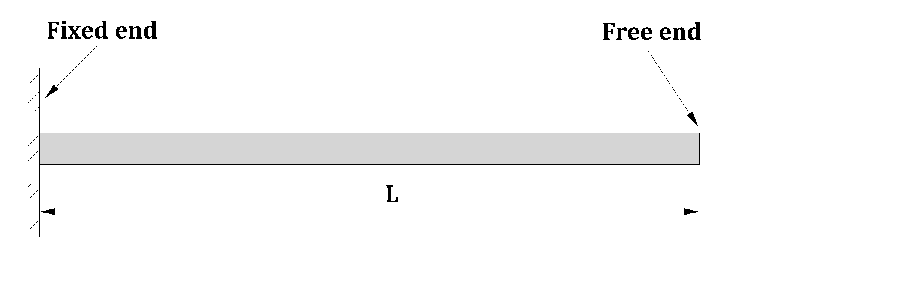
\includegraphics[width=0.6\textwidth]{./PICS/AxBar_PDT.pdf}}\\
\subfloat[]{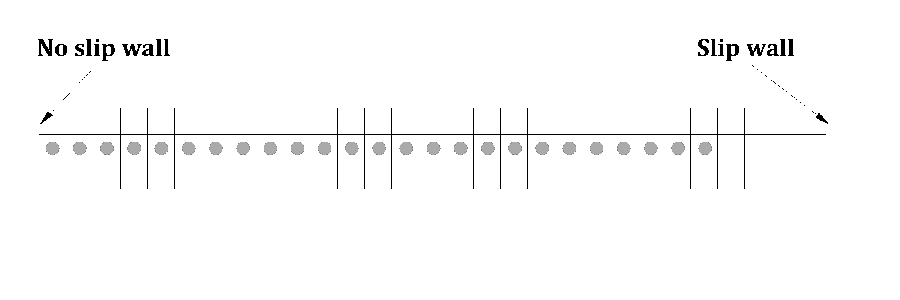
\includegraphics[width=0.6\textwidth]{./PICS/AxBar_PDMPM.pdf}}
\caption{Axial vibration of bar. (a) Configuration of test case (b) Corresponding MPM modeling. Gray lines indicate the background Eulerian grid and the gray circles are the material points located at time $t=0$}
\label{Fig:TestCaseAxBar}
\end{figure}
The test case configuration is shown in Figure~\ref{Fig:TestCaseAxBar}(a). The bar has a length $L$ with an area of cross-section $A$ and is made up of a linear elastic material with Young's modulus $E$. The poisson's ratio of the material is set as zero. The bar is fixed at one end and left free at the other. The equation governing the vibration of the bar is given by,
\begin{align}
	\frac{\partial^2 u}{\partial t^2}=c^2 \frac{\partial^2 u}{\partial x^2}
\label{Eq:goveq_axial_bar}
\end{align}
where $u$ is the axial displacement and $c$ is the speed of sound in the elastic medium. The bar is subjected to the following boundary conditions as previously explained. 
\begin{align}
	u(0,t)=0\\
	\frac{\partial u}{\partial x} (L,t) = 0
\end{align}
When an initial axial velocity $v(x,0)= V_0 \sin \left(\frac{\pi x}{2 L}\right)$ is imposed on the bar, the full exact solution to the governing equation Eq~\ref{Eq:goveq_axial_bar} is given by,
\begin{align}
& u(x, t)=\frac{V_0}{\omega_1} \sin \left(\frac{\pi x}{2 L}\right) \sin \left(\omega_1 t\right) \\
& v(x, t)=V_0 \sin \left(\frac{\pi x}{2 L}\right) \cos \left(\omega_1 t\right)
\end{align}
where $\omega_1$ is the fundamental frequency of the first mode of vibration.
%Explanation on the numerical set up.

Numerical simulations of this test case is performed using \Ex solver. The properties of the bar are set as $E=100, L=25$ and $V_0 = 0.1$.  The density of the material, $\rho$ is set equal to unity. The length of the bar is descretized using $25$ material points located equidistant from each other. A three-dimensional, structured background grid is chosen in this study with grid edge of unit length.  The grid has three cells each in both the lateral dimensions and $29$ grid cells in the longitudinal direction such that at the initial time each material point is located at the center of the cell as shown in Figure~\ref{Fig:TestCaseAxBar}(b). Four grid cells are left as a buffer region between the right most material point and the right boundary of the background grid. No-slip and slip wall boundary conditions are imposed on the left and the right boundaries respectively while periodic boundary conditions are imposed in the other directions. Simulations are performed using both the linear-hat shape functions as well as the cubic-spline shape functions and for $\alpha_{P-F}$ equal to zero and one respectively. The CFL numbers are also varied $0.01$ to $0.5$ in different simulations. For ease of presentation, the comparisons between the exact solution and the MPM solutions obtained using \Ex are shown here using the center of mass velocity of the bar, $v_{cm}$ and using system energies. The exact center of mass velocity is given by $v_{\mathrm{cm}}^{\mathrm{exa}}(t)=\frac{V_0 c}{\omega_1 L} \cos \left(\omega_1 t\right)$ and its MPM counterpart is calculated as $v_{\mathrm{cm}}^{\mathrm{num}}(t)=\frac{\sum v_p(t) m_p}{\sum m_p}$. Three different forms of system energy is shown for comparison, namely the kinetic energy ($KE=\frac{1}{2} \sum_{p=1}^{n_p} \mathbf{v}_p \cdot \mathbf{v}_p m_p$), the strain energy ($SE=\frac{1}{2} \sum_{p=1}^{n_p} \sigma_{p} \epsilon_{p} V_p$) and the total energy ($TE=KE+SE$).

\subsubsection{Effect of $\alpha_{P-F}$}
Figure~\ref{Fig:TestCaseAxBar_EoA_Vel} shows the variation of $v_{cm}$ as a function of time for two different values of $\alpha_{P-F}$ ($0$ and $1$). It is observed that for $\alpha_{P-F}=0$, the center of mass velocity decreases with time in contrast to the exact solution where the amplitude remains unchanged. On the other hand, for $\alpha_{P-F}=1$ the exact nature of the solution is well captured by MPM solution.

\begin{figure}[h]
\subfloat[$\alpha_{P-F}=0$]{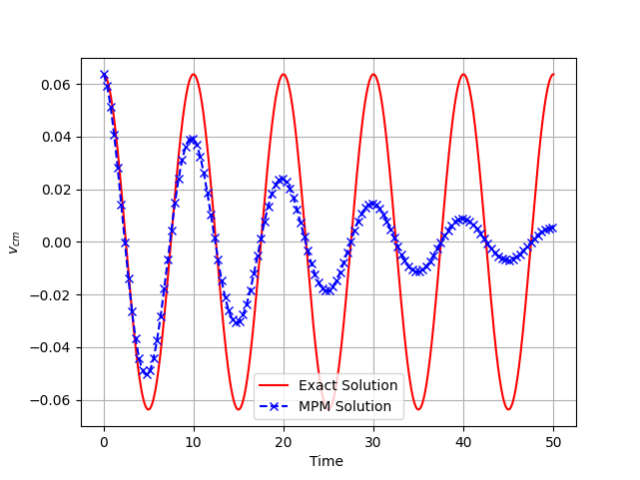
\includegraphics[width=0.4\textwidth]{./PICS/AVB_Effect_of_alpha_Vel_1Order_a=0.png}}
\subfloat[$\alpha_{P-F}=1$]{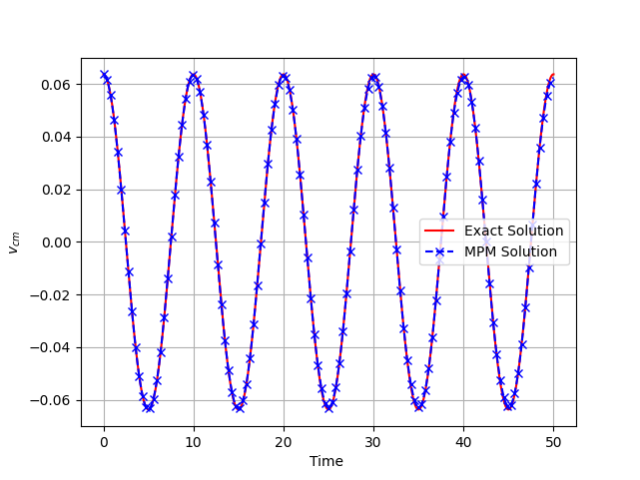
\includegraphics[width=0.4\textwidth]{./PICS/AVB_Effect_of_alpha_Vel_1Order_a=1.png}}
\caption{Exact and MPM computed center of mass velocity $v_{cm}$ as a function of time. Linear hat shape function used with $CFL=0.1$}
\label{Fig:TestCaseAxBar_EoA_Vel}
\end{figure}

This dissipative nature of the numerical solution at low values of $\alpha_{P-F}$ can also be observed from the temporal variation of energy plotted in Figure~\ref{Fig:TestCaseAxBar_EoA_Engy}. Both kinetic and strain energy (and hence the total energy as well) is found to decrease and ultimately reach zero with time for $\alpha_{P-F}=0$ while $\alpha_{P-F}=1$ captures the non-dissipative nature of the exact solution accurately.

\begin{figure}[h]
\subfloat[$\alpha_{P-F}=0$]{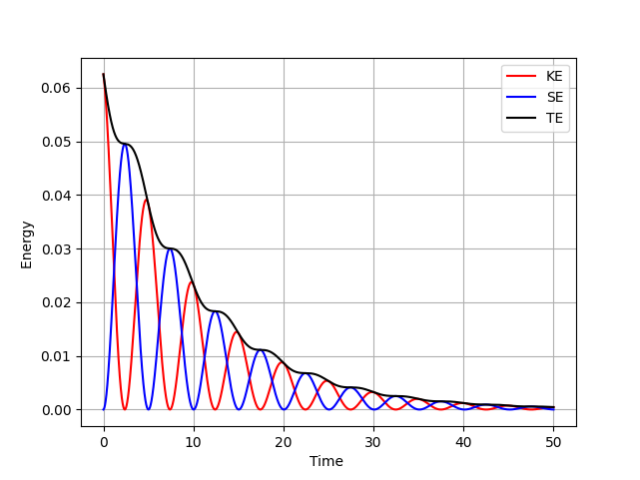
\includegraphics[width=0.3\textwidth]{./PICS/AVB_Effect_of_alpha_Engy_1Order_a=0.png}}
\subfloat[$\alpha_{P-F}=1$]{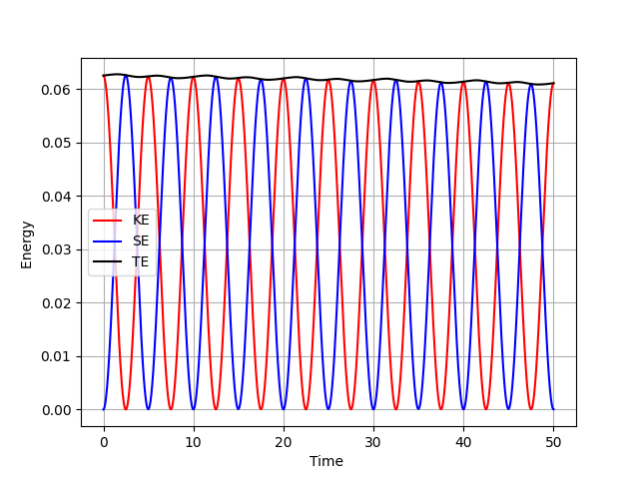
\includegraphics[width=0.3\textwidth]{./PICS/AVB_Effect_of_alpha_Engy_1Order_a=1.png}}
\caption{Exact and MPM computed energy  as a function of time. Linear hat shape function used with $CFL=0.1$}
\label{Fig:TestCaseAxBar_EoA_Engy}
\end{figure}

\subsubsection{Effect of $CFL$}
It is also interesting to study the effect of $CFL$ on the solution accuracy. Figure~\ref{Fig:TestCaseAxBar_EoCFL_CS_a0} shows the time evolution of $v_{cm}$ for values of $CFL=0.01,0.1$ and $0.5$. The results shown are obtained using the cubic spline shape functions and for $\alpha_{P-F}=0$. It is observed that the MPM solution deviates from the exact one as the $CFL$ is reduced. The solution is observed to be more dissipative as the CFL number is reduced. Results obtained using the linear hat shape function also show a similar trend and hence are not shown here.

\begin{figure}[h]
\subfloat[$CFL=0.01$]{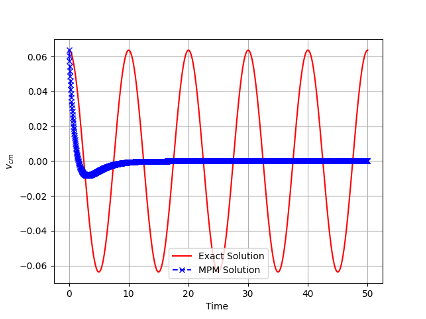
\includegraphics[width=0.3\textwidth]{./PICS/AVB_Effect_of_CFL_Vel_3Order_a=0_CFL_0p01.png}}
\subfloat[$CFL=0.1$]{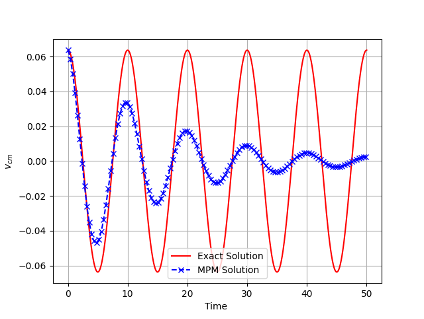
\includegraphics[width=0.3\textwidth]{./PICS/AVB_Effect_of_CFL_Vel_3Order_a=0_CFL_0p1.png}}
\subfloat[$CFL=0.5$]{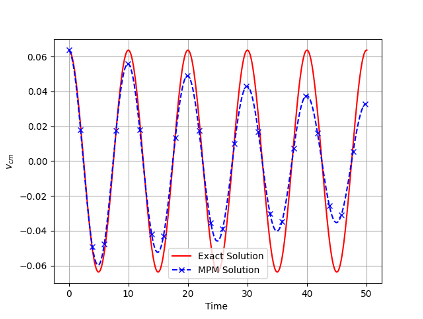
\includegraphics[width=0.3\textwidth]{./PICS/AVB_Effect_of_CFL_Vel_3Order_a=0_CFL_0p5.png}}
\caption{Exact and MPM center of mass velocity $v_{cm}$ as a function of time computed using cubic spline shape function.$\alpha_{P-F}=0$}
\label{Fig:TestCaseAxBar_EoCFL_CS_a0}
\end{figure}

On the contrary, very minimal deviations from exact solution are observed for all $CFL$ numbers for  $\alpha_{P-F}=1$ as shown in Figure~\ref{Fig:TestCaseAxBar_EoCFL_CS_a1}. Same trend also holds for solution computed using the linear hat shape function as well.

\begin{figure}[h]
\subfloat[$CFL=0.01$]{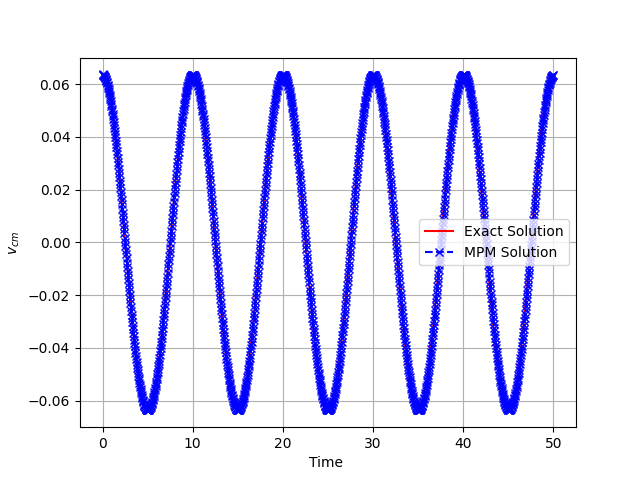
\includegraphics[width=0.3\textwidth]{./PICS/AVB_Effect_of_CFL_Vel_3Order_a=1_CFL_0p01.png}}
\subfloat[$CFL=0.1$]{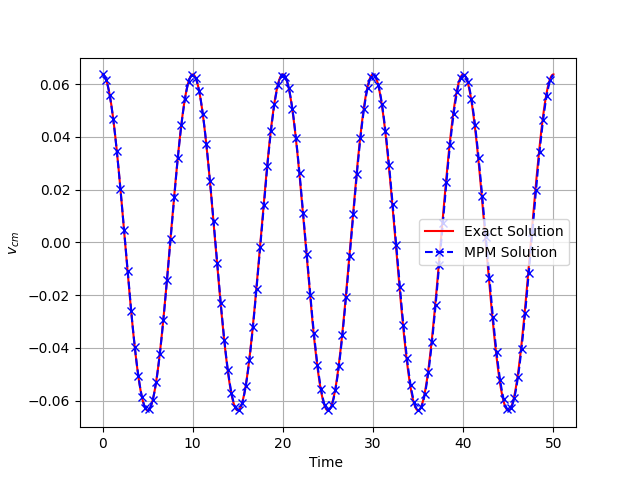
\includegraphics[width=0.3\textwidth]{./PICS/AVB_Effect_of_CFL_Vel_3Order_a=1_CFL_0p1.png}}
\subfloat[$CFL=0.5$]{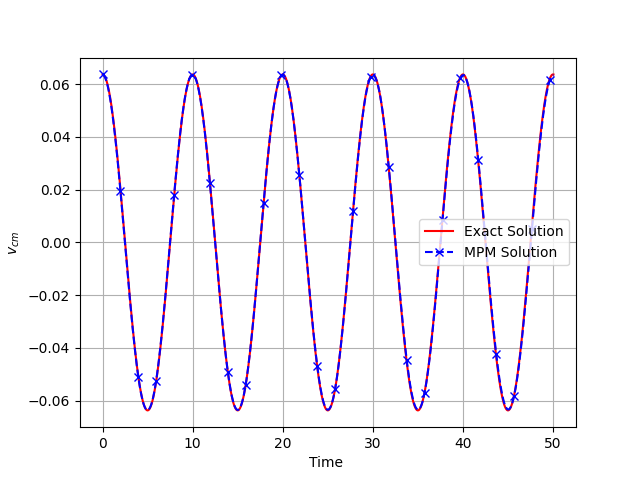
\includegraphics[width=0.3\textwidth]{./PICS/AVB_Effect_of_CFL_Vel_3Order_a=1_CFL_0p5.png}}
\caption{Exact and MPM center of mass velocity $v_{cm}$ as a function of time computed using cubic spline shape function.$\alpha_{P-F}=1$}
\label{Fig:TestCaseAxBar_EoCFL_CS_a1}
\end{figure}

Hence, it is concluded that lower values of $\alpha_{P-F}$ lead to dissipative solution. The dissipative nature further worsens for smaller values of CFL number as well. Hence, for all MPM simulations a typical value of $\alpha_{P-F}=0.95-1.0$ is used.


\subsection{Collision of two-dimensional elastic disks}
This test case is used to verify the \Ex capability to detect and simulate problems with collision. This two-dimensional test case configuration is shown in Figure~\ref{Fig:TestCaseEDC}(a) and consists of two elastics disks each of radius $r$ and separated by a distance $d$. At time $t=0$, both the disks have a velocity $v$ and move towards each other. As time progresses both the disks approach closer to each other at constant velocity and collide. After collision, the disks rebound and move away from each other. Since the collision is elastic, the total energy of the disks remain constant in time.

For simulating this test case in \Ex, the value of Young's modulous $E$ and density $\rho$ is chosen as $1000$. The poissons ratio is set as 0.3. The radius of the disks is set to 0.2 m each and the disks are separated by a distance $d=0.6\sqrt{2}$. The background grid is a square grid of side $L=2$m and consists of 20 cells each in the x and y directions. The two disks are modeled using linear elastic material points with four of them located inside each cell. Simulations are carried out using both the linear hat and the cubic spline shape functions. Based on the conclusions from the previous test case, the value of CFL and  $\alpha_{P-F}$ is chosen as 0.1 and 0.95 respectively. 

\begin{figure}[h]
\subfloat[]{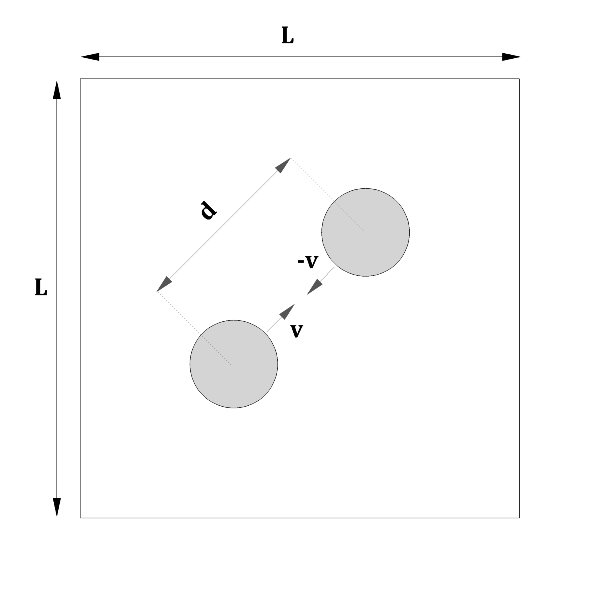
\includegraphics[width=0.35\textwidth]{./PICS/EDC_PDT.pdf}}
\subfloat[]{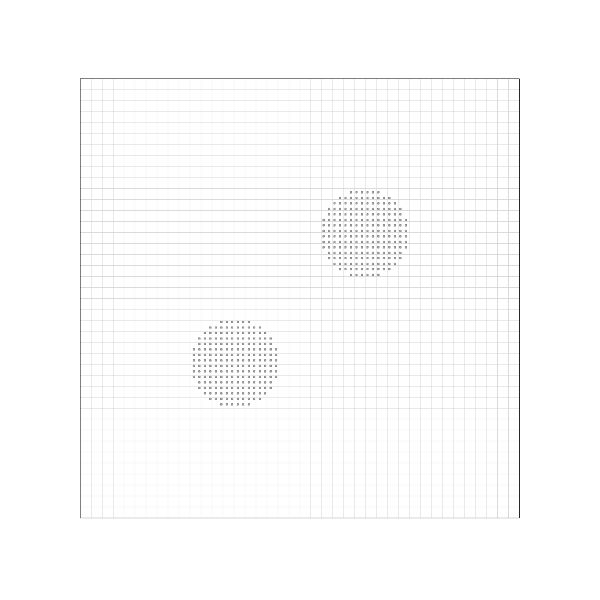
\includegraphics[width=0.35\textwidth]{./PICS/EDC_PDMPM.pdf}}
\caption{(a) Problem definition of the elastic collision of disks test case. (b) MPM background grid and disks modeled through material points}
\label{Fig:TestCaseEDC}
\end{figure}

Figures~\ref{Fig:TestCaseEDC_Res1}(a) and (b) show the approach of the disks towards each other.  Figures~\ref{Fig:TestCaseEDC_Res1}(c) shows the instant at which the disks collide and (d) shows the disks rebounding after collision. 

\begin{figure}[h]
\subfloat[$t=0$]{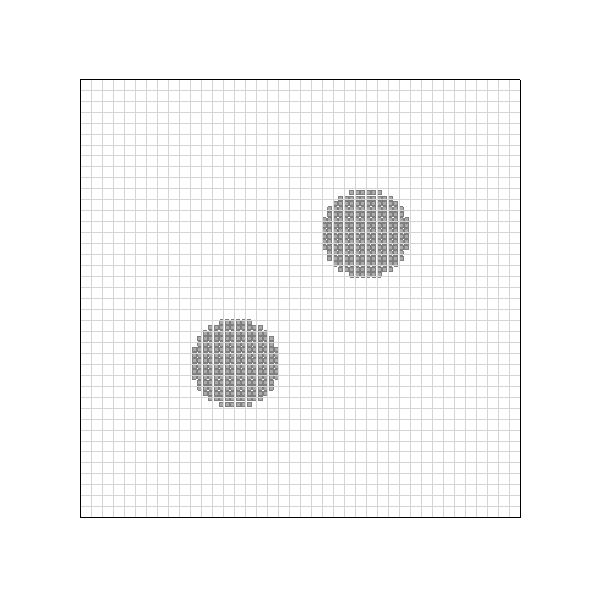
\includegraphics[width=0.2\textwidth]{./PICS/EDC1.pdf}}
\subfloat[$t=0.85$]{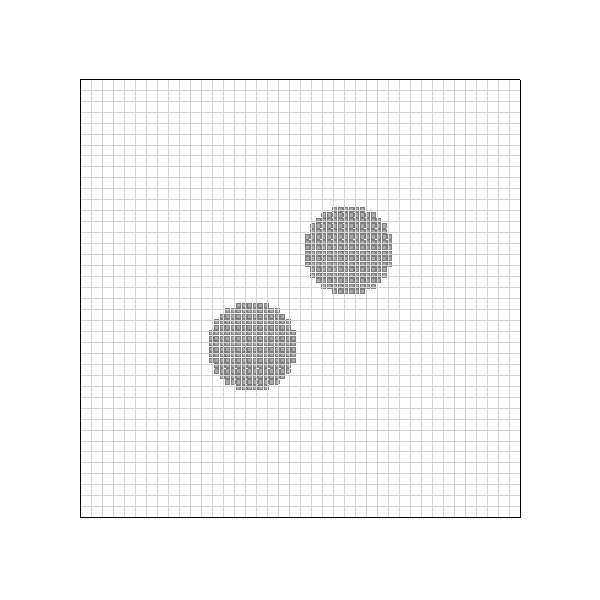
\includegraphics[width=0.2\textwidth]{./PICS/EDC2.pdf}}
\subfloat[$t=2.25$]{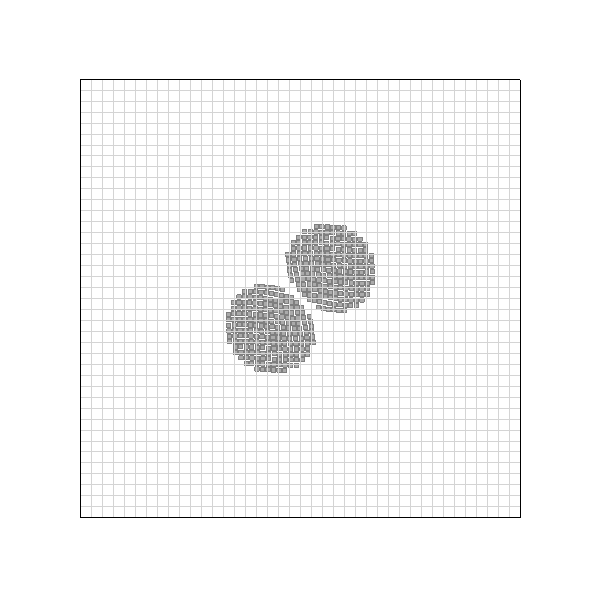
\includegraphics[width=0.2\textwidth]{./PICS/EDC3.pdf}}
\subfloat[$t=3.1$]{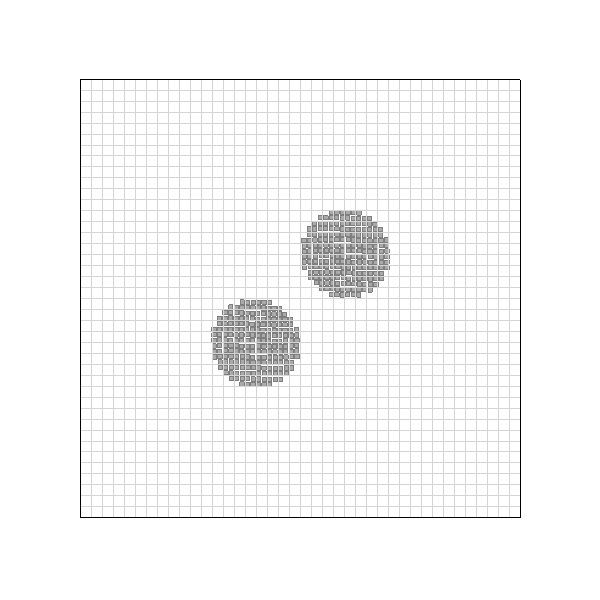
\includegraphics[width=0.2\textwidth]{./PICS/EDC4.pdf}}
\caption{Disks motion at various instants of time}
\label{Fig:TestCaseEDC_Res1}
\end{figure}

Figures~\ref{Fig:TestCaseEDC_Res2}(a) and (b) show the evolution of the energies with time calculated using linear hat and cubic spline shape functions. At initial time and till the time of collision, there is only kinetic energy for both the disks due to the initial velocities. 

\begin{figure}[h]
\subfloat[Linear hat shape function]{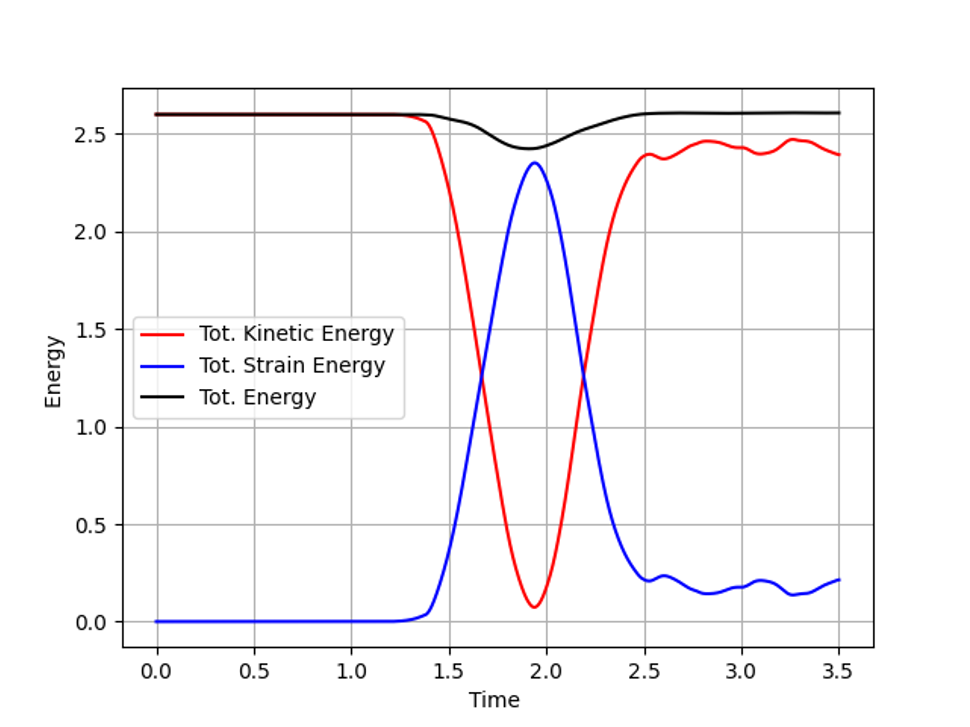
\includegraphics[width=0.35\textwidth]{./PICS/EDC_Energy_LH.png}}
\subfloat[Cubic spline shape function]{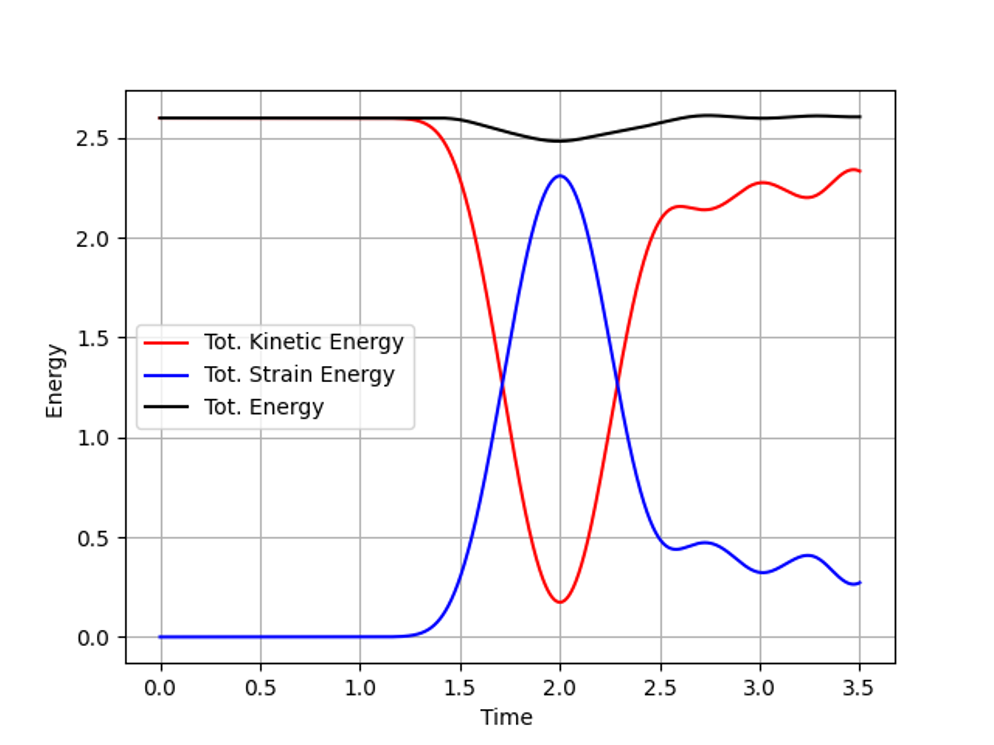
\includegraphics[width=0.35\textwidth]{./PICS/EDC_Energy_CS.png}}
\caption{Evolution of the kinetic, strain and total energies of the disks}
\label{Fig:TestCaseEDC_Res2}
\end{figure}

Once the disks collide, a portion of the total energy is converted to strain energy. Since there are no dissipative mechanisms modeled in this problem, the total energy of the disks should be conserved. Both the linear hat and the cubic spline shape function is able to recover the total energy completely. A temporary loss of total energy is observed during the time of collision. This is due to the mass lumping algorithm adopted which tend to make the solution slightly dissipative. The exact time of contact happens at time $t=1.58$sec while the numerical simulations tend to predict the contact much early. This is because, the contact in MPM occurs through the background grid nodes and not through material points. This inaccuracy can be reduced by refining the background grid further.

\subsection{Dam break simulation}
To demonstrate the application of \Ex solver to simulate flow of fluids, dam break simulation is carried out. The test case consists of a column of water of height $H_0$ and width $L_0$ located inside a square domain, at time $t=0$. For $t>0$, the water column is left free and flows down due to gravity. Water fills up the entire domain as time progresses. Experimental measurement of the water front is available \cite{martin1952} for comparison with MPM results. 

For MPM simulations, the domain is chosen as shown in Figure~\ref{Fig:TestCaseDB}(b). A square domain of side 0.4m is chosed for creating the background grid. The square grid is descretized using 100 cells in each direction. The height of the water column is chosen as 0.2m and the width as 0.1m. Contrary to the previous test cases discussed, water is treated as a fluid and requires specification of an equation of state. In this study, water is modelled using a barotopic equation of state that relates pressure to the density of water as,
\begin{align}
p=\kappa\left[\left(\frac{\rho}{\rho_0}\right)^\gamma-1\right]
\end{align}
The value of $\kappa$ and $\gamma$ is set as 20000 and 7.0 respectively. The density of water is initialised as 1000 kg/m3. Simulation is performed using $CFL=0.1$ and $\alpha_{P-F}=0.95$. The spatial descretization scheme used is that of cubic-spline. The simulation snapshot at various instants of time as shown in Figure~\ref{Fig:TestCaseDB_Res1}. 


\begin{figure}[tbh]
\subfloat[Problem definition of dam break test case]{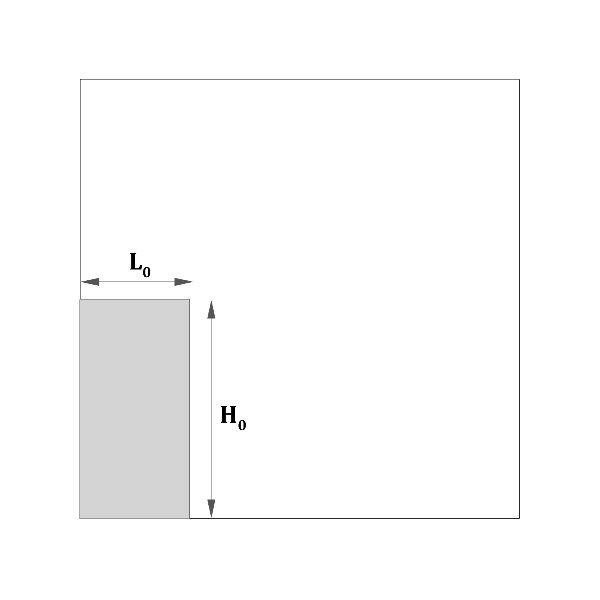
\includegraphics[width=0.4\textwidth]{./PICS/DB_PDT.pdf}}
\subfloat[MPM modeling of dam break case]{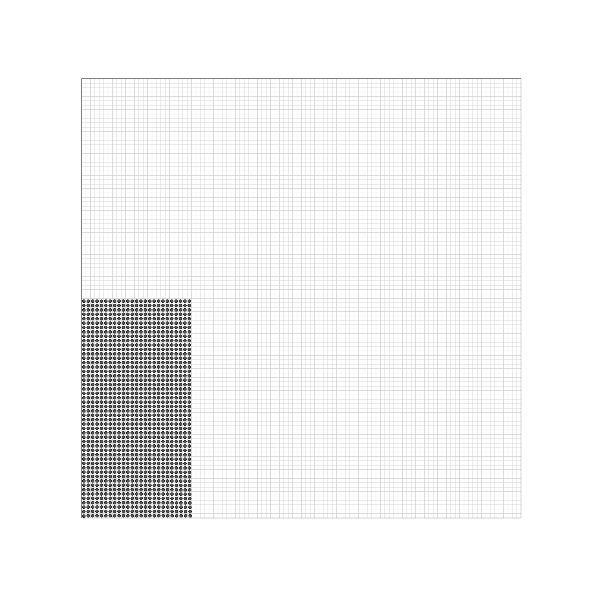
\includegraphics[width=0.4\textwidth]{./PICS/DB1.pdf}}\\
\caption{Dam break test case}
\label{Fig:TestCaseDB}
\end{figure}

\begin{figure}[h]
\subfloat[$t=0.0$]{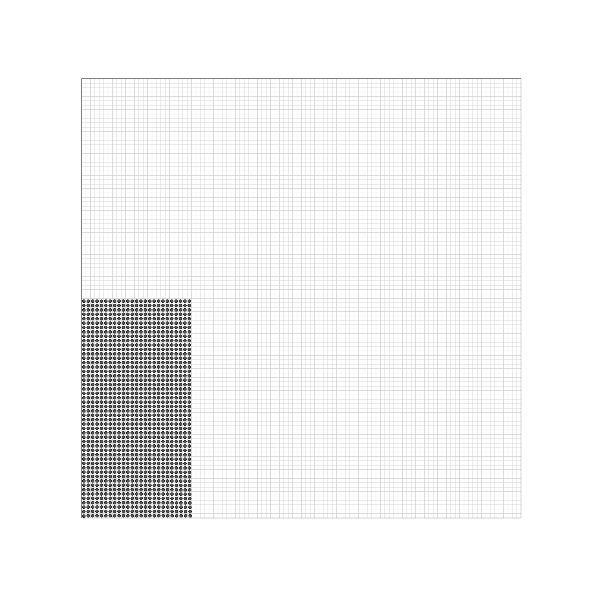
\includegraphics[width=0.25\textwidth]{./PICS/DB1.pdf}}
\subfloat[$t=0.15$]{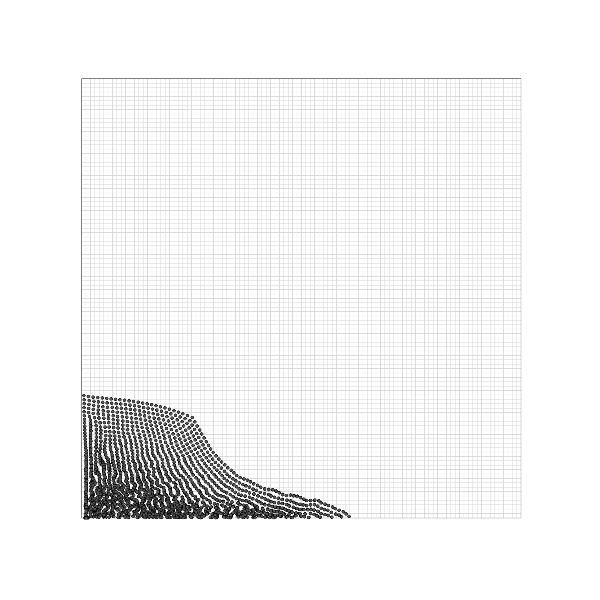
\includegraphics[width=0.25\textwidth]{./PICS/DB2.pdf}}
\subfloat[$t=0.22$]{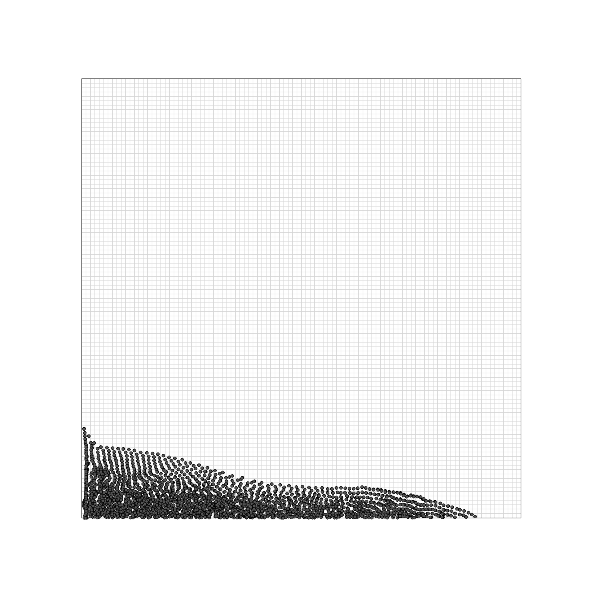
\includegraphics[width=0.25\textwidth]{./PICS/DB3.pdf}}
\subfloat[$t=0.29$]{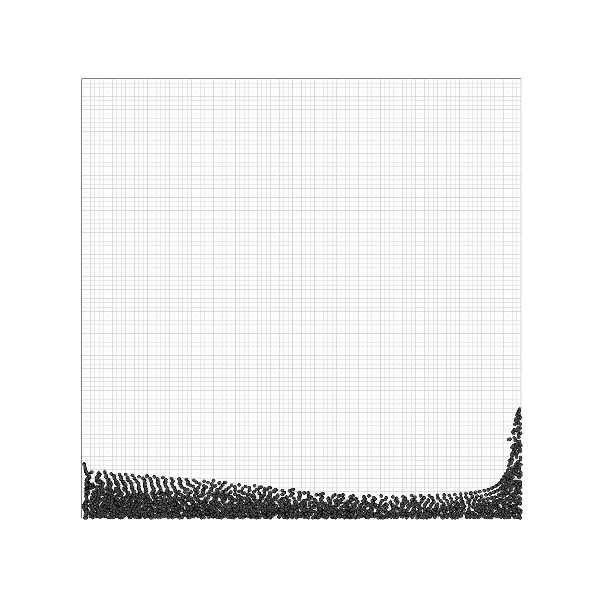
\includegraphics[width=0.25\textwidth]{./PICS/DB4.pdf}}
\caption{Water front movement at various instants of time}
\label{Fig:TestCaseDB_Res1}
\end{figure}

Figure~\ref{Fig:TestCaseDB_Res2} shows a comparison of the water front calculated using \Ex and experimentally obtained water front values \cite{martin1952} at various times. A good comparison is obtained between the numerical and experimental values thereby validating the solver.

\begin{figure}[h]
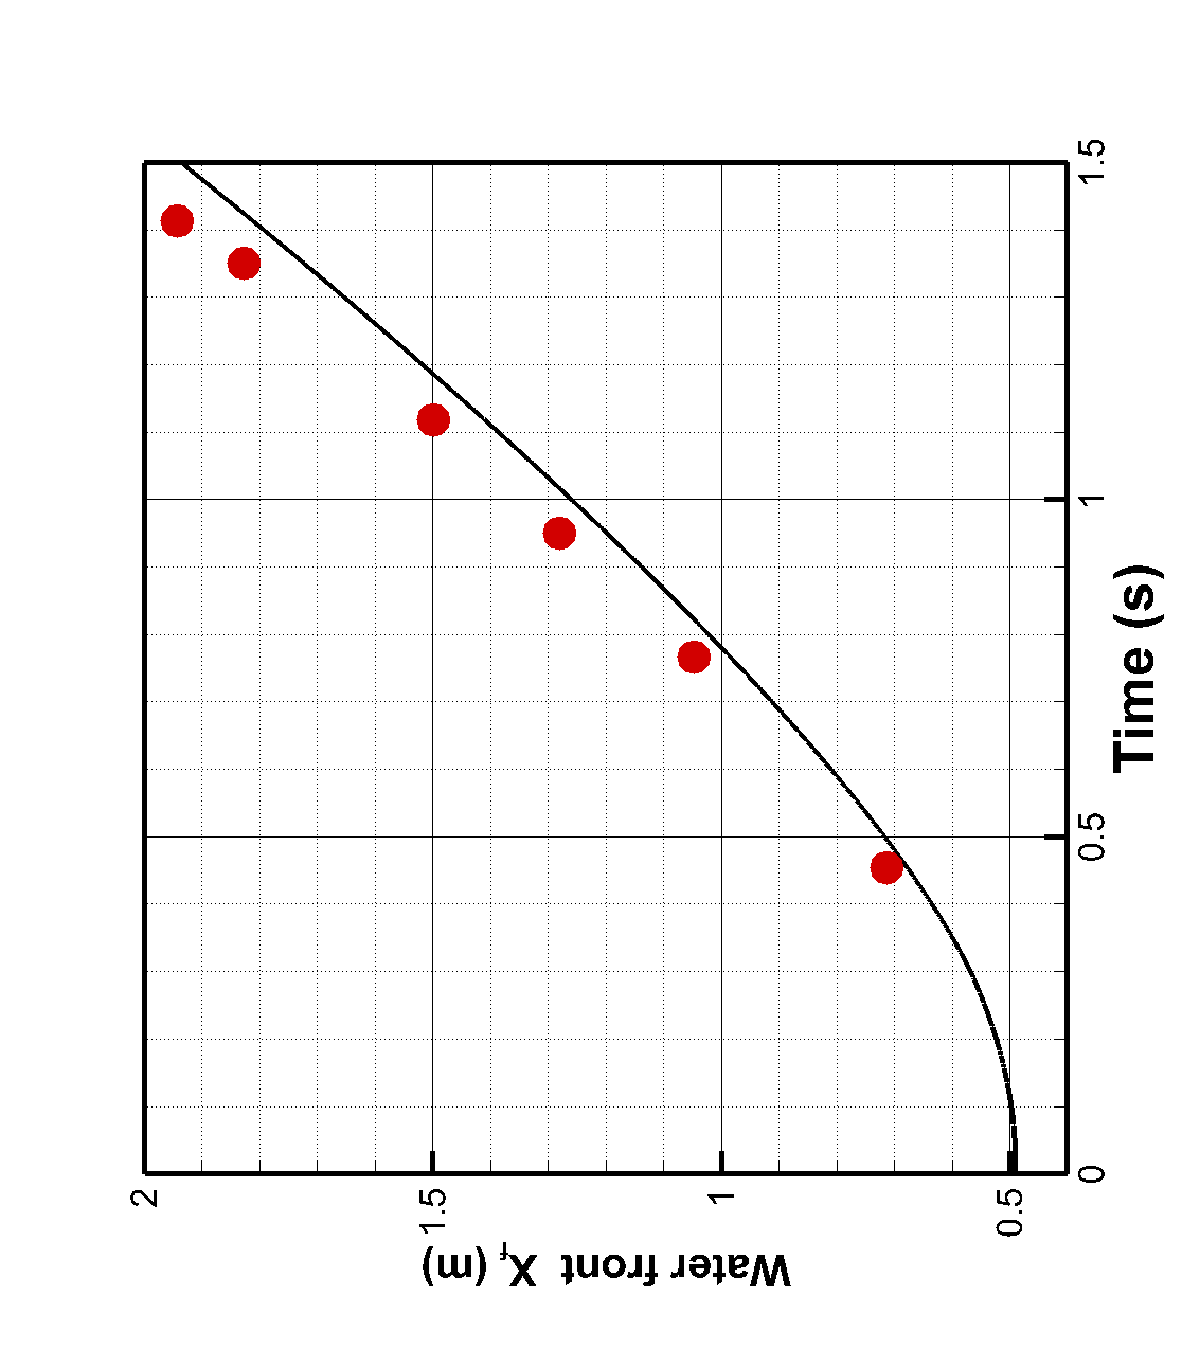
\includegraphics[width=0.4\textwidth, angle =-90]{./PICS/DB_Res2.pdf}
\caption{Time evolution of water front location. Line is MPM solution and circles indicate experimental data from \cite{martin1952}}
\label{Fig:TestCaseDB_Res2}
\end{figure}
